\documentclass[12pt,a4paper]{article}
\usepackage{setspace}
\usepackage[T1]{fontenc}
\usepackage[utf8]{inputenc}
\IfFileExists{newtxtext.sty}{\usepackage{newtxtext}}{\usepackage{mathptmx}}
\usepackage[a4paper,left=1.75cm,right=1.75cm,top=61.2pt,bottom=70pt,
            headheight=14pt,headsep=33.8pt,footskip=51.4pt]{geometry}
\usepackage{xcolor}
\usepackage{graphicx}
\usepackage{array}
\usepackage{tabularx}
\usepackage{fancyhdr}
\usepackage{eso-pic}
\usepackage{ragged2e}
\usepackage{url}

% ---------- colours (sampled from the template) ----------
\definecolor{gebanner}{RGB}{0,102,148}
\definecolor{gegold}{RGB}{255,201,38}
\definecolor{geheading}{RGB}{43,91,145}
\definecolor{gehint}{gray}{0.5}

% ---------- edit these once ----------
\newcommand{\courseinfo}{DSCPP-III-2026-T272}
\newcommand{\leadname}{Kumar, Tanmay}
\newcommand{\mtwo}{Saxena, Sparsh}
\newcommand{\mthree}{Sethi, Hemang}

% ---------- graphicspath ----------
\graphicspath{{./}{../media/}{media/}}

% ---------- page style: header, page number, gold bar ----------
\pagestyle{fancy}
\fancyhf{}
\renewcommand{\headrulewidth}{0pt}
\fancyhead[L]{\fontsize{10.5}{12.6}\selectfont\courseinfo}
\fancyhead[R]{\fontsize{10.5}{12.6}\selectfont PHASE-III PROJECT PROGRESS\hspace{2.6pt}}
\fancyfoot[R]{\fontsize{10}{12}\selectfont Page \thepage}
\AddToShipoutPictureBG{%
  \AtPageLowerLeft{\color{gegold}\rule{\paperwidth}{4pt}}}

\setlength{\parindent}{0pt}
\setlength{\tabcolsep}{6pt}
\setlength{\topskip}{16.5pt}
\setstretch{1.15}
\renewcommand{\arraystretch}{1}

% ---------- building blocks ----------
\newcommand{\banner}[3]{%
  \noindent\colorbox{gebanner}{\parbox[c][#3][c]{\dimexpr\textwidth-2\fboxsep\relax}{%
    \fontsize{#2}{#2}\selectfont\bfseries\color{gegold}#1}}\par}

\newcommand{\secthead}[2]{%
  {\fontsize{18}{21.9}\selectfont\color{geheading}#1\par}\vspace{1.6pt}%
  {\fontsize{10.5}{14.5}\selectfont\color{gehint}#2\par}%
  \vspace{\secgap}}
\newlength{\secgap}\setlength{\secgap}{5.7pt}
\newcommand{\afterbox}{\vspace{\aftergap}}
\newlength{\aftergap}\setlength{\aftergap}{12pt}

\newcolumntype{R}[1]{>{\RaggedRight\arraybackslash}p{#1}}
\newenvironment{answerbox}{%
  \noindent\begin{tabular}{|p{\dimexpr\textwidth-2\tabcolsep-2\arrayrulewidth\relax}|}\hline
  \fontsize{10.8}{13.3}\selectfont\setlength{\parskip}{3.5pt}\rule{0pt}{18pt}\ignorespaces}{%
  \rule[-11pt]{0pt}{0pt}\\\hline\end{tabular}\par}

\newcommand{\tablehead}[1]{\fontsize{12}{14.5}\selectfont\bfseries #1}
\newcommand{\tablebody}{\fontsize{11}{13.6}\selectfont\rule[-5.5pt]{0pt}{19pt}}

\begin{document}

% ============================================================
% PAGE 1: PROJECT AND TEAM INFORMATION
% ============================================================

\vspace*{-0.35cm}


\includegraphics[width=7.5cm,height=1.7cm,keepaspectratio]{geulogo.png}

\vspace{0.20cm}

\banner{PROJECT AND TEAM INFORMATION}{16.5}{24pt}

\vspace{0.20cm}

\secthead{Project Title}{(Try to choose a catchy title. Max 20 words).}

\begin{answerbox}
\textbf{Maze Lab: Real-Time Interactive Navigation, Generation and Comparative Pathfinding}
\end{answerbox}

\vspace{0.25cm}

\noindent
\renewcommand{\arraystretch}{1.0}
\begin{tabularx}{\textwidth}{|>{\RaggedRight\arraybackslash}p{0.48\textwidth}|>{\RaggedRight\arraybackslash}X|}
\hline
\begin{minipage}[c][1.20cm][c]{\linewidth}
\textit{Team Name:}\\[1.2mm]
\textit{Team \#}
\end{minipage}
&
\begin{minipage}[c][1.20cm][c]{\linewidth}
\textit{Team Blockbuster}\\[1.2mm]
\textit{T272}
\end{minipage}
\\
\hline
\begin{minipage}[c][5.05cm][t]{\linewidth}
\vspace*{2.5mm}
\textbf{Team member 1 (Team Lead)}\\[1.5mm]
{\color{gehint}\fontsize{10}{12.5}\selectfont(Last Name, name: student ID: email, picture):}\\
\end{minipage}
&
\begin{minipage}[c][5.05cm][t]{\linewidth}
\vspace*{2mm}
\fontsize{10.5}{12.5}\selectfont
\textit{\leadname\ -- 2510370439}\\
\textit{2510370439@geu.ac.in}\\[2mm]
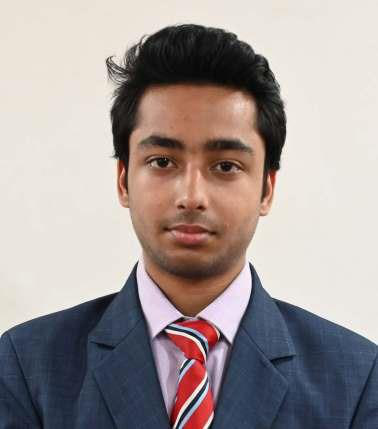
\includegraphics[width=5.4cm,height=3.55cm,keepaspectratio]{media/Tanmay.png}
\end{minipage}
\\
\hline
\begin{minipage}[c][5.05cm][t]{\linewidth}
\vspace*{2.5mm}
\textbf{Team member 2}\\[1.5mm]
{\color{gehint}\fontsize{10}{12.5}\selectfont(Last Name, name: student ID: email, picture):}\\
\end{minipage}
&
\begin{minipage}[c][5.05cm][t]{\linewidth}
\vspace*{2mm}
\fontsize{10.5}{12.5}\selectfont
\textit{\mtwo\ -- 2510370313}\\
\textit{2510370313@geu.ac.in}\\[2mm]
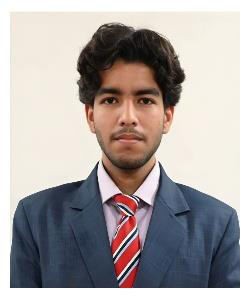
\includegraphics[width=5.4cm,height=3.55cm,keepaspectratio]{media/Sparsh.png}
\end{minipage}
\\
\hline
\begin{minipage}[c][5.05cm][t]{\linewidth}
\vspace*{2.5mm}
\textbf{Team member 3}\\[1.5mm]
{\color{gehint}\fontsize{10}{12.5}\selectfont(Last Name, name: student ID: email, picture):}\\
\end{minipage}
&
\begin{minipage}[c][5.05cm][t]{\linewidth}
\vspace*{2mm}
\fontsize{10.5}{12.5}\selectfont
\textit{\mthree\ -- 2510370341}\\
\textit{2510370341@geu.ac.in}\\[2mm]
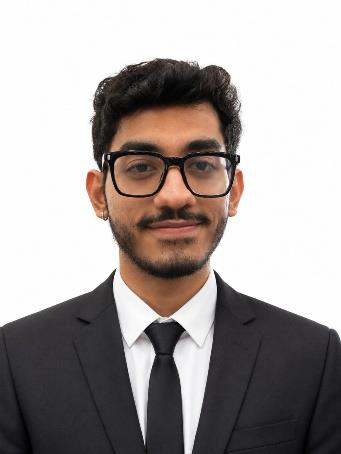
\includegraphics[width=5.4cm,height=3.55cm,keepaspectratio]{media/Hemang.png}
\end{minipage}
\\
\hline
\end{tabularx}
\renewcommand{\arraystretch}{1}

\newpage

% ============================================================
% PAGE 2: PROGRESS DESCRIPTION
% ============================================================
\vspace*{-0.15cm}

\banner{PHASE-III PROJECT PROGRESS DESCRIPTION (35 pts)}{16.5}{26pt}

\vspace{0.30cm}

\secthead{Project Abstract }{(Brief restatement of your project's main goal. Max 300 words).}

\begin{answerbox}
Maze Lab is a high-performance ISO C++17 application combining foundational Data Structures with Object-Oriented Programming (OOP) principles to construct, traverse, and solve 2D mazes algorithmically. The project supports real-time interactive gameplay for human players with instant key response alongside automated solvers to benchmark manual navigation against graph search strategies. Perfect, loop-free mazes are generated using either Iterative Randomized Depth-First Search (DFS) or Randomized Kruskal's algorithm via a custom Disjoint Set Union (DSU) data structure. Autonomous shortest-path finding is performed using Breadth-First Search (BFS) and A* search guided by an admissible Manhattan distance heuristic. The Strategy Pattern decouples both generation and solving engines, enabling runtime algorithmic selection without modifying core grid logic. Phase III marks 100\% completion, delivering real-time non-blocking WASD controls, step-by-step console animations, an optional zero-dependency native GUI built directly on the Win32 API (Windows) and \texttt{libX11} (Linux), and an automated benchmarking engine tracking path length, explored node counts, and execution times.
\end{answerbox}

\afterbox

\secthead{Updated Project Approach and Architecture }{(Describe your current approach, including system design, communication protocols, libraries used, etc. Max 300 words).}

\begin{answerbox}
The system models a maze as a 2D matrix of \texttt{Cell} objects owned by a centralized \texttt{Maze} container, where each cell tracks coordinates, visited state, and four directional walls. All wall removals are routed through \texttt{Maze::openPassage()} to guarantee symmetric, bidirectional updates without boundary desynchronization. Graph-theoretically, cells represent vertices and carved passages form unit-weight undirected edges.\par\vspace{2pt}
Architectural modularity follows the Strategy Pattern through abstract interfaces \texttt{MazeGenerator} and \texttt{MazeSolver}, implemented by \texttt{DFSGenerator}, \texttt{KruskalGenerator}, \texttt{BFSSolver}, and \texttt{AStarSolver}. The \texttt{Player} class encapsulates position updates, step tracking, and wall-collision checks. For zero-latency terminal gameplay, raw keyboard input is captured directly via POSIX \texttt{termios} on Linux/WSL and \texttt{\_getch()} on Windows.\par\vspace{2pt}
Each algorithm uses its optimal data structure: iterative DFS relies on a heap-allocated \texttt{std::stack<Coord>} to avoid call-stack overflow; BFS uses \texttt{std::queue<Coord>} with a parent matrix for guaranteed shortest paths; A* employs \texttt{std::priority\_queue} ordered by $f(n) = g(n) + h(n)$ with Manhattan distance; and Kruskal's algorithm applies a custom DSU (path compression and union-by-rank) over shuffled right/bottom walls. All solvers return a unified \texttt{SolveResult} struct recording path length, visited nodes, and \texttt{<chrono>} runtime. Presentation supports both lightweight ANSI console rendering and an optional platform-native GUI built on the Win32 API (\texttt{gdi32}/\texttt{user32}) for Windows and Xlib (\texttt{libX11}) for Linux via compile-time platform guards, eliminating external graphics library dependencies.
\end{answerbox}

\newpage

% ============================================================
% PAGE 3: TASKS COMPLETED & CHALLENGES
% ============================================================

\vspace*{-0.15cm}

\secthead{Tasks Completed }{(Describe the main tasks that have been assigned and already completed. Max 250 words).}

{\fontsize{10.5}{12.8}\selectfont
\renewcommand{\arraystretch}{1.06}
\begin{tabularx}{\textwidth}{
|>{\raggedright\arraybackslash}X
|>{\raggedright\arraybackslash}p{0.34\textwidth}|
}
\hline
\textbf{Task Completed} & \textbf{Team Member} \\
\hline
Cell and Maze classes (2D grid, centralized wall logic) & Tanmay Kumar \\
\hline
Abstract MazeGenerator and MazeSolver strategy interfaces & Tanmay Kumar \\
\hline
Iterative Randomized DFS generator with explicit stack & Sparsh Saxena \\
\hline
BFS pathfinding solver with parent tracking & Sparsh Saxena \\
\hline
Disjoint Set Union (DSU) data structure & Hemang Sethi \\
\hline
Randomized Kruskal's maze generator implementation & Hemang Sethi \\
\hline
A* pathfinder with Manhattan distance heuristic & Sparsh Saxena \\
\hline
Real-time WASD input handler (\texttt{termios} / \texttt{\_getch()}) & Hemang Sethi \\
\hline
ANSI console animation \& native Win32/\texttt{libX11} GUI renderer & Hemang Sethi \\
\hline
Metrics engine (steps, nodes explored, microsecond timing) & Tanmay Kumar \\
\hline
Comparative analysis menu (BFS vs A* side-by-side run) & Sparsh Saxena \\
\hline
End-to-end integration and main menu loop & Tanmay Kumar \\
\hline
Test suite, validation, and Phase-III report & All members \\
\hline
\end{tabularx}
\renewcommand{\arraystretch}{1}
}

\afterbox

\secthead{Challenges/Roadblocks }{(Describe the challenges that you have faced or are facing so far and how you plan to solve them. Max 300 words).}

\begin{answerbox}
\textbf{Bidirectional Wall Inconsistency:} Editing adjacent cell walls independently caused unilateral passage bugs. Routing all wall removals exclusively through \texttt{Maze::openPassage()} enforced symmetric updates.\par\vspace{2pt}
\textbf{Stack Overflow in Large Grids:} Recursive DFS risks exhausting the call stack on large grids (e.g., $50 \times 50$). Converting DFS into an iterative algorithm backed by a heap-allocated \texttt{std::stack<Coord>} resolved this completely.\par\vspace{2pt}
\textbf{Duplicate Edges in Kruskal's Algorithm:} Naive wall iteration doubles internal edges because neighbors share boundaries. Collecting only right and bottom internal walls per cell produced an exact, duplicate-free edge list.\par\vspace{2pt}
\textbf{Cross-Platform Input \& Native GUI Portability:} Standard \texttt{std::cin} introduced Enter-key latency, while bundling heavy third-party GUI toolkits complicated compilation. We abstracted raw-mode keyboard input (POSIX \texttt{termios} on Linux, \texttt{\_getch()} on Windows) and built a zero-dependency native GUI directly on the Win32 API (Windows) and \texttt{libX11} (Linux) behind preprocessor guards.\par\vspace{2pt}
\textbf{Objective Solver Benchmarking:} Standardizing solver output via a shared \texttt{SolveResult} struct and isolating \texttt{<chrono>} timing from UI rendering ensured fair BFS vs. A* comparisons.
\end{answerbox}

\newpage

% ============================================================
% PAGE 4: OUTCOMES & PROGRESS OVERVIEW
% ============================================================

\vspace*{-0.15cm}

\secthead{Project Outcome/Deliverables (2 pts)}{(Describe what are the key outcomes / deliverables of the project. Max 200 words).}

\begin{answerbox}
The primary outcome of Phase III is a self-contained, fully validated ISO C++17 software application demonstrating practical OOP architecture and graph algorithms. Specific deliverables include: (1) two perfect-maze generators implementing Iterative Randomized DFS and Randomized Kruskal's algorithm with Disjoint Set Union; (2) two optimal pathfinding solvers comprising Breadth-First Search and A* search with an admissible Manhattan heuristic; (3) a real-time interactive play mode featuring non-blocking WASD controls and wall-collision validation; (4) a unified benchmarking engine measuring path length, explored node counts, and sub-millisecond runtimes; (5) dual visualization modes combining an animated ANSI console renderer with a native cross-platform GUI built on the Win32 API (Windows) and \texttt{libX11} (Linux); and (6) a version-controlled GitHub repository containing modular source code, automated validation tests, build instructions, and the final Phase-III project report.
\end{answerbox}

\afterbox

\secthead{Progress Overview (2 pts)}{(Summarize how much of the project is done, what's behind schedule, what's ahead of schedule. Max 200 words.)}

\begin{answerbox}
With the completion of Phase III, the Maze Lab project is 100\% complete, with zero tasks behind schedule. Every core algorithmic module carried forward from Phase II---specifically Randomized Kruskal's generator with custom DSU, the A* heuristic pathfinder, and the unified BFS vs. A* benchmarking suite---has been fully implemented, integrated, and validated. Beyond the baseline Phase-I specification, real-time single-key navigation, animated console pathfinding, and optional platform-native GUI rendering (Win32 API on Windows and \texttt{libX11} on Linux) were delivered ahead of schedule to elevate usability and visual clarity. Empirical benchmarks confirm that A* substantially reduces explored node counts compared to BFS while guaranteeing identical optimal path lengths. All source files, validation checks, and Phase-III evaluation documents are finalized and ready for live demonstration.
\end{answerbox}

\newpage

% ============================================================
% PAGE 5: CODEBASE, TESTING & DELIVERABLES STATUS
% ============================================================

\vspace*{-0.15cm}

\secthead{Codebase Information }{(Repository link, branch, and information about important commits.)}

\begin{answerbox}
\textbf{Repository:} \url{https://github.com/Tanmay-git65/III-SEM-PBL} \hfill \textbf{Branch:} \texttt{master}\\[2.5pt]
\textbf{Important Commits:}\\[1pt]
\textbullet\ \texttt{b09bbff} -- Project repository initialization and directory layout\\
\textbullet\ \texttt{9cea4fb} -- Core Maze model, iterative DFS generator, and BFS solver (Phase II)\\
\textbullet\ \texttt{eef6b70} -- Architecture documentation, design specifications, and technical notes\\
\textbullet\ \texttt{61aa4fa} -- Cross-platform builds and raw terminal input integration\\
\textbullet\ \texttt{Phase-III} -- Kruskal (DSU), A* solver, Win32/\texttt{libX11} GUI, and benchmarking suite
\end{answerbox}

\vspace{10pt}

\secthead{Testing and Validation Status }{(Provide information about any tests conducted)}

{\fontsize{10.2}{12.2}\selectfont
\renewcommand{\arraystretch}{1.04}
\begin{tabularx}{\textwidth}{
|>{\raggedright\arraybackslash}p{0.34\textwidth}
|>{\raggedright\arraybackslash}p{0.15\textwidth}
|>{\raggedright\arraybackslash}X|
}
\hline
\textbf{Test Type} & \textbf{Status} & \textbf{Notes} \\
\hline
DFS Maze Connectivity & Pass & All cells reachable; verified loop-free spanning tree. \\
\hline
Kruskal Maze Connectivity & Pass & DSU cycle prevention; fully connected spanning tree. \\
\hline
Player Wall Collision & Pass & Invalid moves into walls or outer bounds rejected. \\
\hline
BFS Path Optimality & Pass & Recovers guaranteed shortest path from start to goal. \\
\hline
A* Path Validity \& Optimality & Pass & Matches BFS optimal length with fewer visited nodes. \\
\hline
Comparative Benchmarking & Pass & Accurate node counts and \texttt{<chrono>} timings recorded. \\
\hline
Cross-Platform UI \& Input & Pass & Verified WASD input, ANSI console, Win32 \& \texttt{libX11} GUI. \\
\hline
\end{tabularx}
\renewcommand{\arraystretch}{1}
}

\vspace{10pt}

\secthead{Deliverables Progress }{(Summarize the current status of all key project deliverables mentioned earlier. Indicate whether each deliverable is completed, in progress, or pending.)}

{\fontsize{10.2}{12.2}\selectfont
\renewcommand{\arraystretch}{1.03}
\begin{tabularx}{\textwidth}{
|>{\raggedright\arraybackslash}X
|>{\raggedright\arraybackslash}p{0.28\textwidth}|
}
\hline
\textbf{Deliverable} & \textbf{Status} \\
\hline
Randomized DFS Generator (Iterative Stack) & Completed \\
\hline
BFS Pathfinder with Parent Tracking & Completed \\
\hline
Disjoint Set Union (DSU) Data Structure & Completed \\
\hline
Randomized Kruskal's Maze Generator & Completed \\
\hline
A* Pathfinder (Manhattan Heuristic) & Completed \\
\hline
Real-Time Interactive WASD Play Mode (\texttt{termios} / \texttt{\_getch()}) & Completed \\
\hline
Animated ANSI Console Pathfinding Visualizer & Completed \\
\hline
Optional Native Cross-Platform GUI (Win32 API \& \texttt{libX11}) & Completed \\
\hline
Metrics and BFS vs A* Comparative Engine & Completed \\
\hline
Comprehensive Validation Suite & Completed \\
\hline
Phase-III Project Progress Report & Completed \\
\hline
\end{tabularx}
\renewcommand{\arraystretch}{1}
}

\end{document}